\documentclass[11pt,letterpaper,titlepage,en-US]{article}

\usepackage{basicstyle}
\usepackage{homework}
\usepackage{weiwBTree}
\usepackage{tikz-qtree}

%
% Homework Details
%   - Title
%   - Due date
%   - Class
%   - Section/Time
%   - Instructor
%   - Author
%


\newcommand{\hmwkTitle}{Homework\ \#5 }
\DTMsavetimestamp{DueDate}{2016-11-20T23:59:59-06:00}
\newcommand{\hmwkClass}{CS 6360.003}
\newcommand{\hmwkClassName}{Database Design}
\newcommand{\hmwkClassInstructor}{Nurcan Yuruk}
\newcommand{\hmwkAuthorName}{Hanlin He}
\newcommand{\hmwkAuthorNetID}{hxh160630}
\newcommand{\hmwkAuthorUTDEmail}{\href{mailto:hanlin.he@utdallas.edu}{hanlin.he@utdallas.edu}}


%
% Title Page
%

\title{
    \vspace{2in}
    \textmd{\textbf{\hmwkClassName \\\hmwkClass:\ \hmwkTitle}}\\
    \normalsize\vspace{0.1in}\small{Due\ on\ \DTMusedate{DueDate}\ at \DTMusetime{DueDate} }\\
    \vspace{0.1in}\large{\textit{\hmwkClassInstructor}}
    \vspace{3in}
}

\author{\textbf{\hmwkAuthorName\ \footnotesize{(\hmwkAuthorNetID)}} \\ \hmwkAuthorUTDEmail}
\date{}

\begin{document}
\maketitle


\pagebreak


\begin{homeworkProblem}
\begin{homeworkSubProblem}
    The record size in bytes is:
    \[R = 30 + 10 + 10 + 30 + 10 + 10 + 1 + 4 + 4 + 1 = 110\text{ bytes. }\]
\end{homeworkSubProblem}

\begin{homeworkSubProblem}
    The blocking factor is:
    \[bfr = \bigg\lfloor\frac{512}{110}\bigg\rfloor = 4\text{ records per block. }\]

    The number of blocks needed assuming an unspanned organization is:
    \[b = \bigg\lceil\frac{3000}{4}\bigg\rceil = 750 \text{ file blocks. }\]
\end{homeworkSubProblem}

\begin{homeworkSubProblem}
    \begin{enumerate}[label=(\roman*)]
        \item Index size is $10+6=16$ bytes, so the index blocking factor is
            \[bfr_i = \bigg\lfloor\frac{512}{16}\bigg\rfloor = 32
            \text{ index records per block. }\]
        \item Total $750$ first level index entries (the same as file blocks),
            so the number of blocks needed for first level index is:
            \[b_i = \bigg\lceil\frac{750}{32}\bigg\rceil = 24 \text{ first level index blocks. }\]
        \item The second level need only $1$ block to store $24$ first level
            index blocks information. Thus, in total, $2$ levels of indexes
            is needed.
        \item Total number of blocks by multi-level index is $1 + 24 = 25$.
        \item $3$ block accesses are needed.
    \end{enumerate}
\end{homeworkSubProblem}

\begin{homeworkSubProblem}
    \begin{enumerate}[label=(\roman*)]
        \item Index size is $10+6=16$ bytes, so the index blocking factor is
            \[bfr_i = \bigg\lfloor\frac{512}{16}\bigg\rfloor = 32
            \text{ index records per block. }\]
        \item Total $3000$ first level index entries (the same as file records),
            so the number of blocks needed for first level index is:
            \[b_i = \bigg\lceil\frac{3000}{32}\bigg\rceil = 94 \text{ first level index blocks. }\]
        \item The second level need $\displaystyle\bigg\lceil\frac{94}{32}\bigg\rceil = 3$
            blocks to store $94$ first level index blocks.\\
            The third level need only $1$ block to store $3$ second level
            index blocks information. Thus, in total, $3$ levels of indexes
            is needed.
        \item Total number of blocks by multi-level index is $1 + 3 + 94 = 98$.
        \item $4$ block accesses are needed.
    \end{enumerate}
\end{homeworkSubProblem}

\begin{homeworkSubProblem}
    \begin{enumerate}[label=(\roman*)]
        \item Index size is $10+6=16$ bytes, so the index blocking factor is
            \[bfr_i = \bigg\lfloor\frac{512}{16}\bigg\rfloor = 32
            \text{ index records per block. }\]
        \item Record pointer size = 7 bytes, thus a block can store
            at most $\displaystyle\bigg\lfloor\frac{512}{7}\bigg\rfloor = 73$
            record pointers. Given $3000$ employees evenly distributed among
            $100$ department, each department has $30$ employees, which is
            smaller than $73$, the capacity of one block to store record pointers,
            i.e. no cluster or linked list is needed.\\
            Thus, $100$ blocks representing $100$ departments by the level
            of indirection are needed.
        \item Total $100$ first level index entries (the same as file blocks),
            so the number of blocks needed for first level index is:
            \[b_i = \bigg\lceil\frac{100}{32}\bigg\rceil = 4 \text{ first level index blocks. }\]
        \item The second level need only $1$ block to store $7$ first level
            index blocks information. Thus, in total, $2$ levels of indexes
            is needed.
        \item Total number of blocks by multi-level index is $1 + 4 = 5$.\\
            The blocks used in the extra level of indirection is $100$.
        \item $3+30=33$ block accesses are needed.
    \end{enumerate}
\end{homeworkSubProblem}

\begin{homeworkSubProblem}
    \begin{enumerate}[label=(\roman*)]
        \item Index size is $10+6=16$ bytes, so the index blocking factor is
            \[bfr_i = \bigg\lfloor\frac{512}{16}\bigg\rfloor = 32
            \text{ index records per block. }\]
        \item $100$ first level index entries representing 100 departments
            are needed.\\
            So the number of blocks needed for first level index is:
            \[b_i = \bigg\lceil\frac{100}{32}\bigg\rceil = 4 \text{ first level index blocks. }\]
        \item The second level need only $1$ block to store $4$ first level
            index blocks information. Thus, in total, $2$ levels of indexes
            is needed.
        \item Each block can store $4$ records, each department has $30$ employees.
            Thus each department needs $\displaystyle\bigg\lceil\frac{30}{4}\bigg\rceil = 8$
            blocks to store all its employees records. In total,
            $8 \times 100 = 800$ blocks is needed. \\
            Total number of blocks by multi-level index is $1 + 4 = 5$.
        \item $2 + 8 = 10$ block accesses are needed.
    \end{enumerate}
\end{homeworkSubProblem}

\begin{homeworkSubProblem}
    \begin{enumerate}[label=(\roman*)]
        \item For B+ tree:
            \begin{align*}
                & (p \times P) + ((p - 1) \times V) \leq B \\
                \Rightarrow\quad & (p \times 6) + ((p - 1) \times 10) \leq 512 \\
                \Rightarrow\quad  & (15 \times p) \leq 522 \\
                \Rightarrow\quad  & \max\{p\} = 32
            \end{align*}
            \begin{align*}
                & (p_{leaf} \times (P_r + V)) + P \leq B \\
                \Rightarrow\quad & (p_{leaf} \times (7 + 10)) + 6 \leq 512 \\
                \Rightarrow\quad  & (17 \times p_{leaf}) \leq 506 \\
                \Rightarrow\quad  & \max\{p_{leaf}\} = 29
            \end{align*}
        \item On the average, each leaf node will hold $0.69 \times p_{leaf} = 0.69 \times 29$
            or approximately 20 data record pointers.\\
            Thus, leaf level blocks number is:
            \[b_{leaf} = \bigg\lceil\frac{3000}{20}\bigg\rceil = 150
            \text{ leaf level blocks. }\]
        \item On the average, each internal node will have
            $0.69 \times p = 0.69 \times 34$ or approximately 22 pointers,
            and hence 21 values.\\
            First internal level blocks number is:
            \[b_1 = \bigg\lceil\frac{150}{21}\bigg\rceil = 8
            \text{ first internal level blocks. }\]
            Second internal level (root level) block number is $1$.\\
            In total, there are $3$ levels.
        \item Total number of blocks required by B+ tree is:
            \[B = 1 + 8 + 150 = 159 \text{ (blocks in total.) }\]
        \item $3 + 1 = 4$ block accesses are needed.
    \end{enumerate}
\end{homeworkSubProblem}

\end{homeworkProblem}


\begin{homeworkProblem}
\begin{figure}[H]
    \caption{Final B+ tree}\label{4}
    \centering
    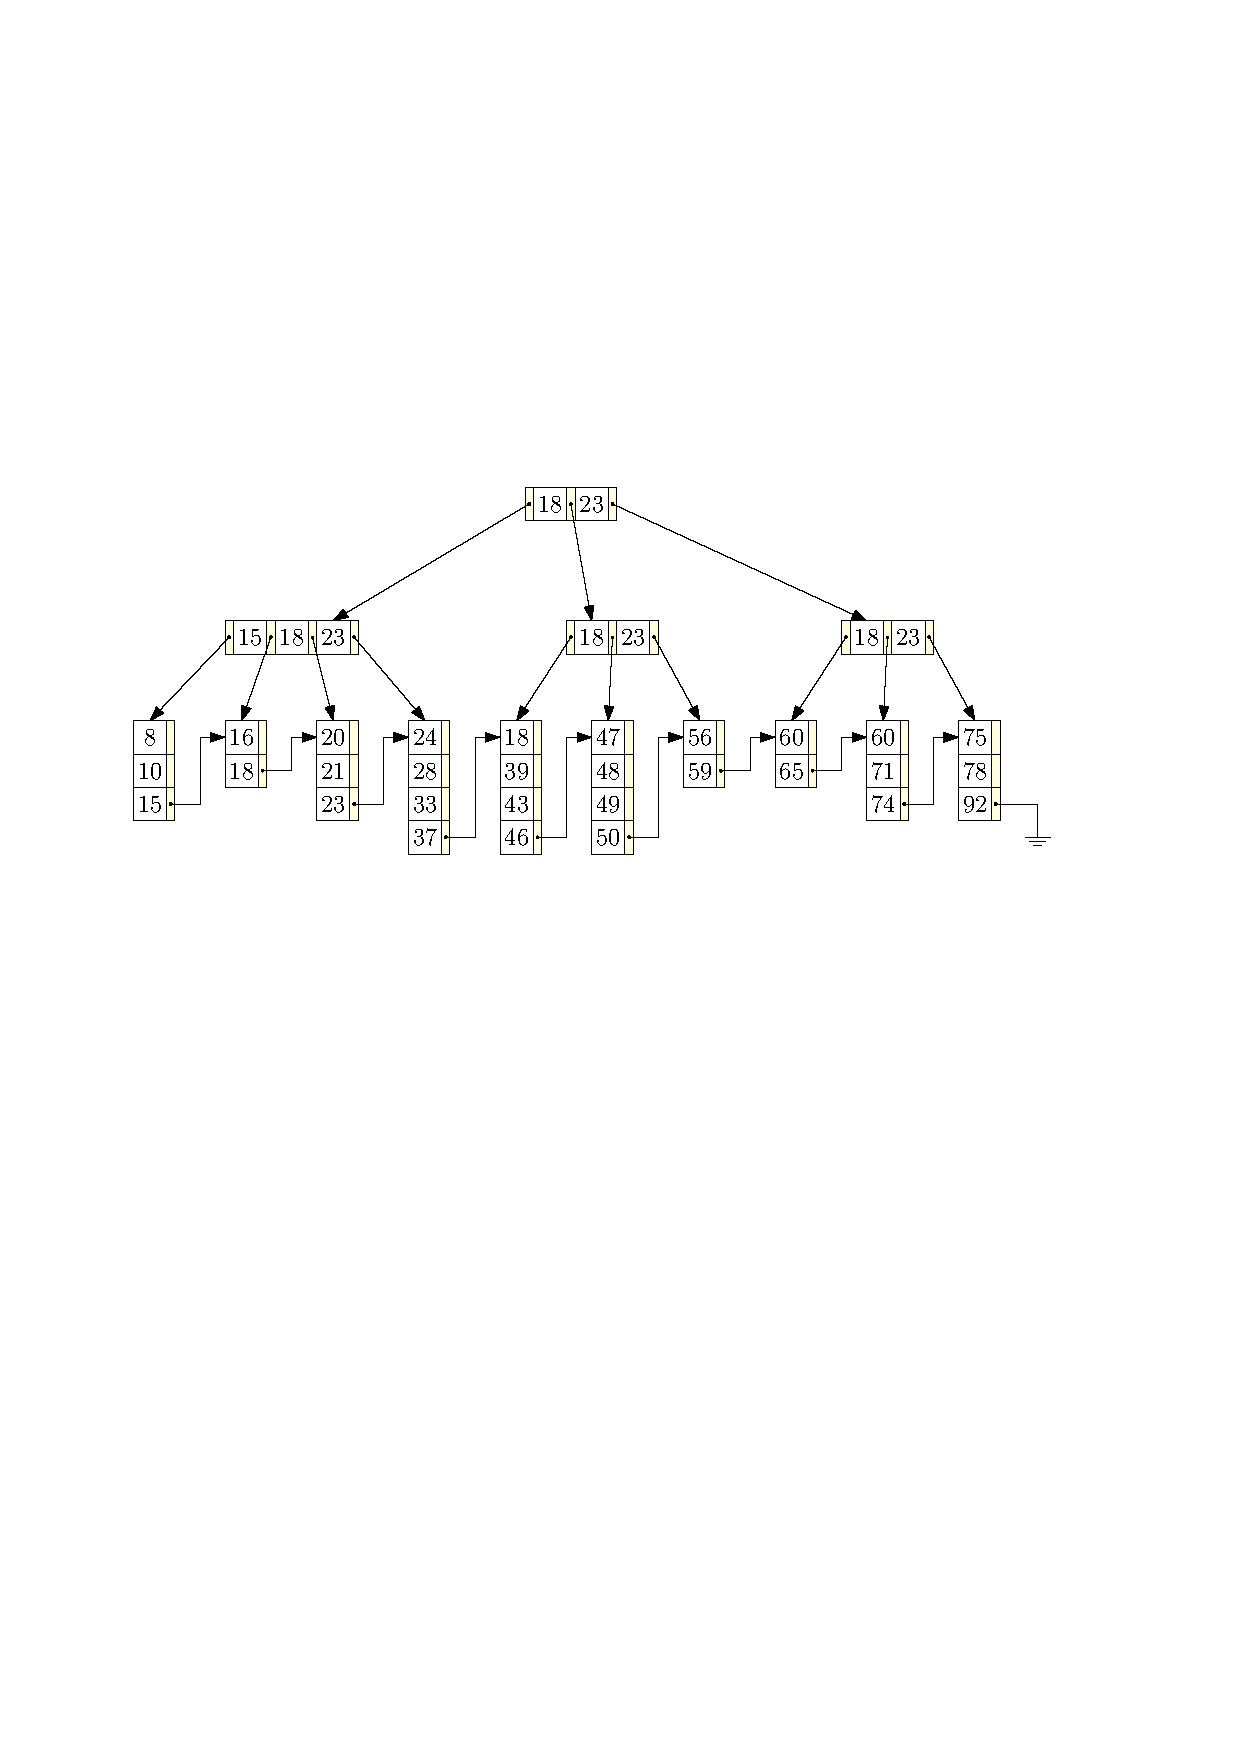
\includegraphics[width=\textwidth]{2}
\end{figure}
\end{homeworkProblem}

\begin{homeworkProblem}

    \tikzset{
        n/.style={draw,circle}
        every tree node/.append style={inner ysep=+0pt,outer ysep=+0pt,minimum size=+0pt}
    }
        \begin{tikzpicture}
            \Tree [.$\pi_{Lname, Fname, Pname, Hours}$
                [.$\bowtie_{E.Ssn = W.Essn}$
                    [.$\pi_{Lname,Fname,Ssn}$
                        [.$\rho_{Salary > 80000}$
                            [.\node[n]{EMPLOYEE}; ]
                        ]
                    ]
                    [.$\pi_{Essn,Hour,Pname}$
                        [.$\bowtie_{P.Pnumber=W.Pno}$ 
                            [.$\pi_{Essn,Pno,Hour}$
                                [.$\rho_{Hour > 30}$
                                    [.WORK\_ON ]
                                ]
                            ]
                            [.$\pi_{Pnumber,Pname}$
                                [.$\bowtie_{P.Dnum = D.Dnumber}$
                                    [.$\pi_{Pnumber,Dnum,Pname}$
                                        [.$\rho_{Plocation='Chicago'}$
                                            [.PROJECT ]
                                        ]
                                    ]
                                    [.$\pi_{Dnumber}$
                                        [.$\rho_{\text{Mgr\_start\_date} \geq \text{'1/1/2009'}}$ 
                                            [.DEPARTMENT ]
                                        ]
                                    ]
                                ]
                            ]
                        ]
                    ]
                ]
            ]
        \end{tikzpicture}
\end{homeworkProblem}


\end{document}
